\begin{table*}[!t]
\begin{center}
\begin{tabular}{llrrr|rrr}
\toprule
           &                & $\delta1 \uparrow$ & $\delta2 \uparrow$ & $\delta3 \uparrow$ & $rel \downarrow$ & $rmse \downarrow$ & $log10 \downarrow$ \\
model & hyperparams &                    &                    &                    &                  &                   &                    \\
\midrule
\multirow{6}{*}{dorn} & CNN &              0.846 &              0.954 &              0.983 &            0.120 &             0.501 &              0.053 \\
           & CNN + median rescaling &              0.871 &              0.964 &              0.988 &            0.111 &             0.473 &              0.048 \\
           & CNN + GT histogram matching &              0.906 &              0.972 &              0.990 &            0.095 &             0.419 &              0.040 \\
           & Ours (SBR=10) &              0.903 &              0.970 &              0.989 &            0.091 &             0.422 &              0.040 \\
           & Ours (SBR=50) &              0.906 &              0.971 &              0.990 &            0.089 &             0.410 &              0.039 \\
           & Ours (SBR=100) &              0.906 &              0.971 &              0.990 &            0.090 &             0.408 &              0.039 \\
\cline{1-8}
\multirow{6}{*}{densedepth} & CNN &              0.847 &              0.973 &              0.994 &            0.123 &             0.461 &              0.053 \\
           & CNN + median rescaling &              0.888 &              0.978 &              0.995 &            0.106 &             0.409 &              0.045 \\
           & CNN + GT histogram matching &              0.930 &              0.984 &              0.995 &            0.079 &             0.338 &              0.034 \\
           & Ours (SBR=10) &              0.922 &              0.982 &              0.994 &            0.082 &             0.361 &              0.036 \\
           & Ours (SBR=50) &              0.925 &              0.983 &              0.995 &            0.081 &             0.348 &              0.035 \\
           & Ours (SBR=100) &              0.926 &              0.983 &              0.995 &            0.081 &             0.346 &              0.035 \\
\bottomrule
\end{tabular}

\caption{Quantitative evaluation using NYU Depth v2. Bold indicates best
performance for that metric, while underline indicates second best. The proposed
scheme outperforms DenseDepth and DORN on all metrics, and it closely matches or
even outperforms the median rescaling scheme and histogram matching with the
exact depth map histogram, even though those methods have access to ground
truth.}
\vspace{-2em}
\label{tab:comparison}
\end{center}
\end{table*}

\begin{figure*}[!h]
  % 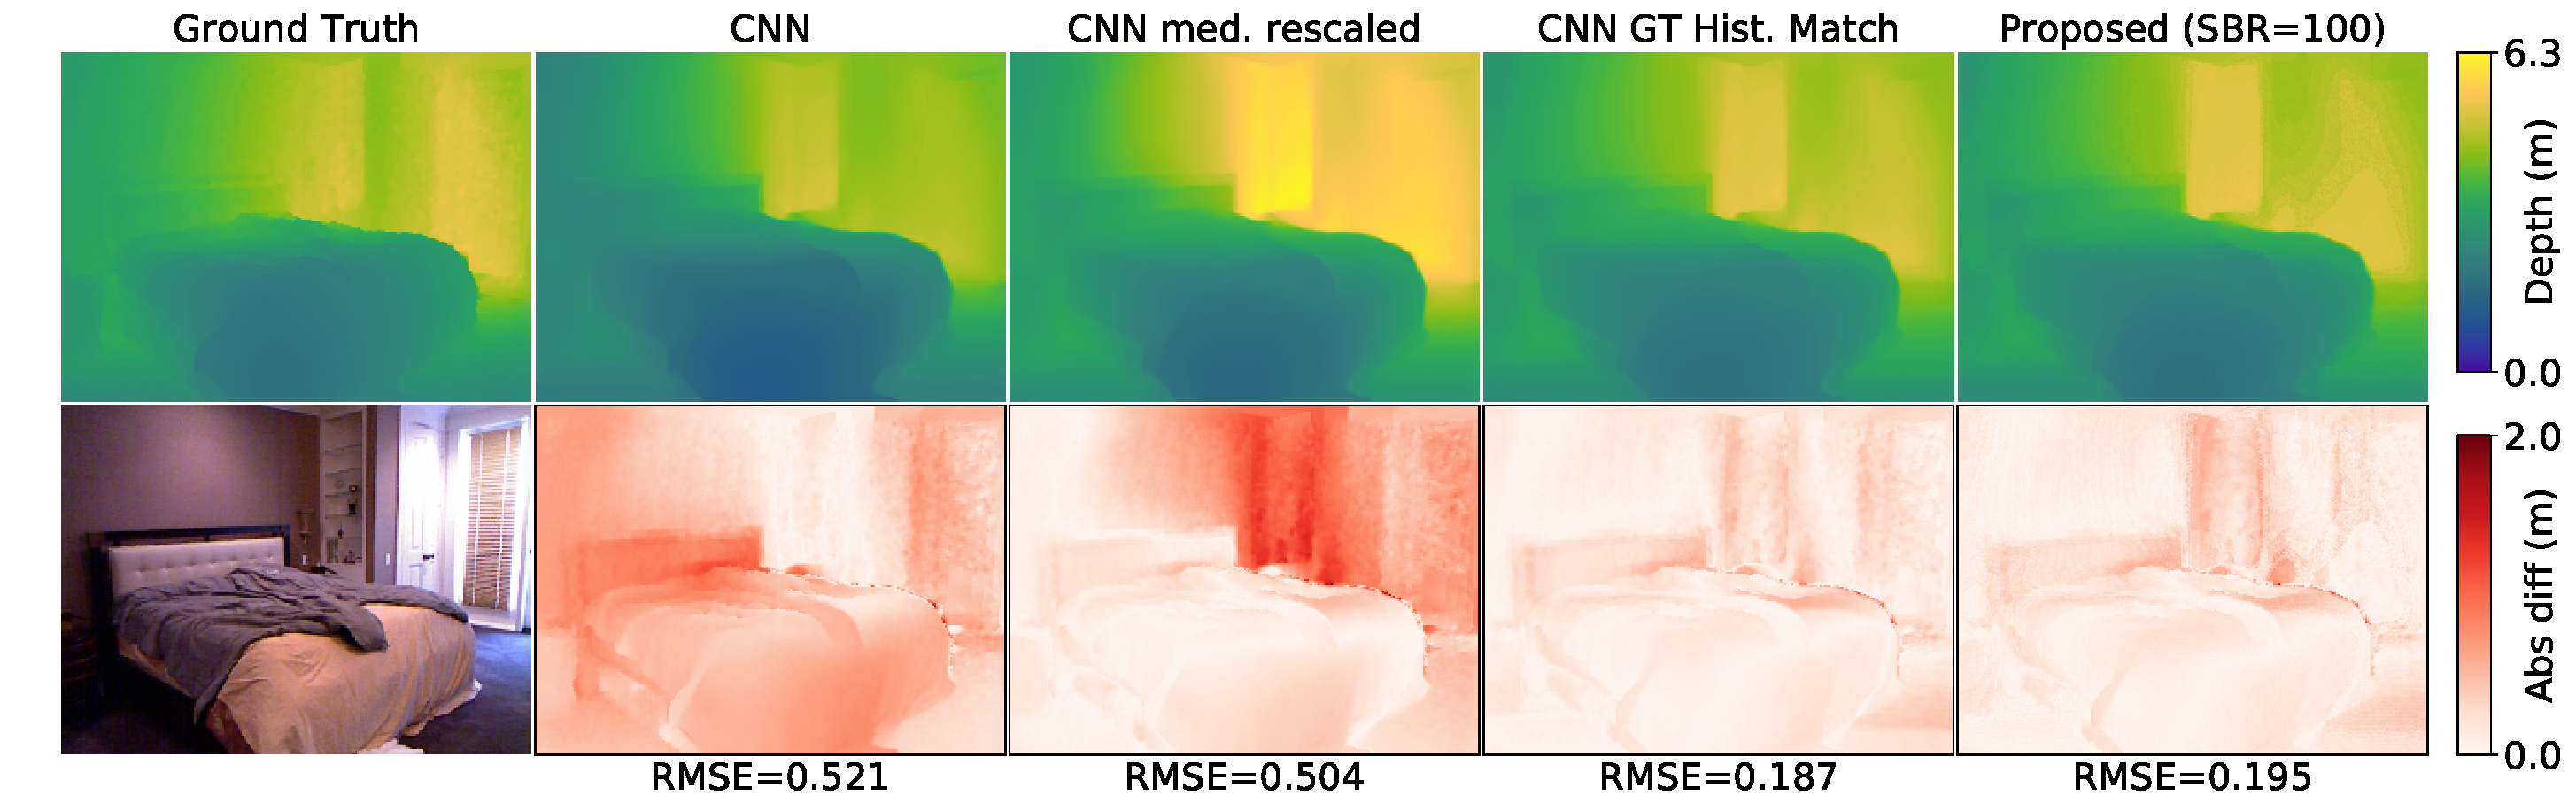
\includegraphics[width=\textwidth]{comparison/densedepth_468_comparison.pdf}
  % 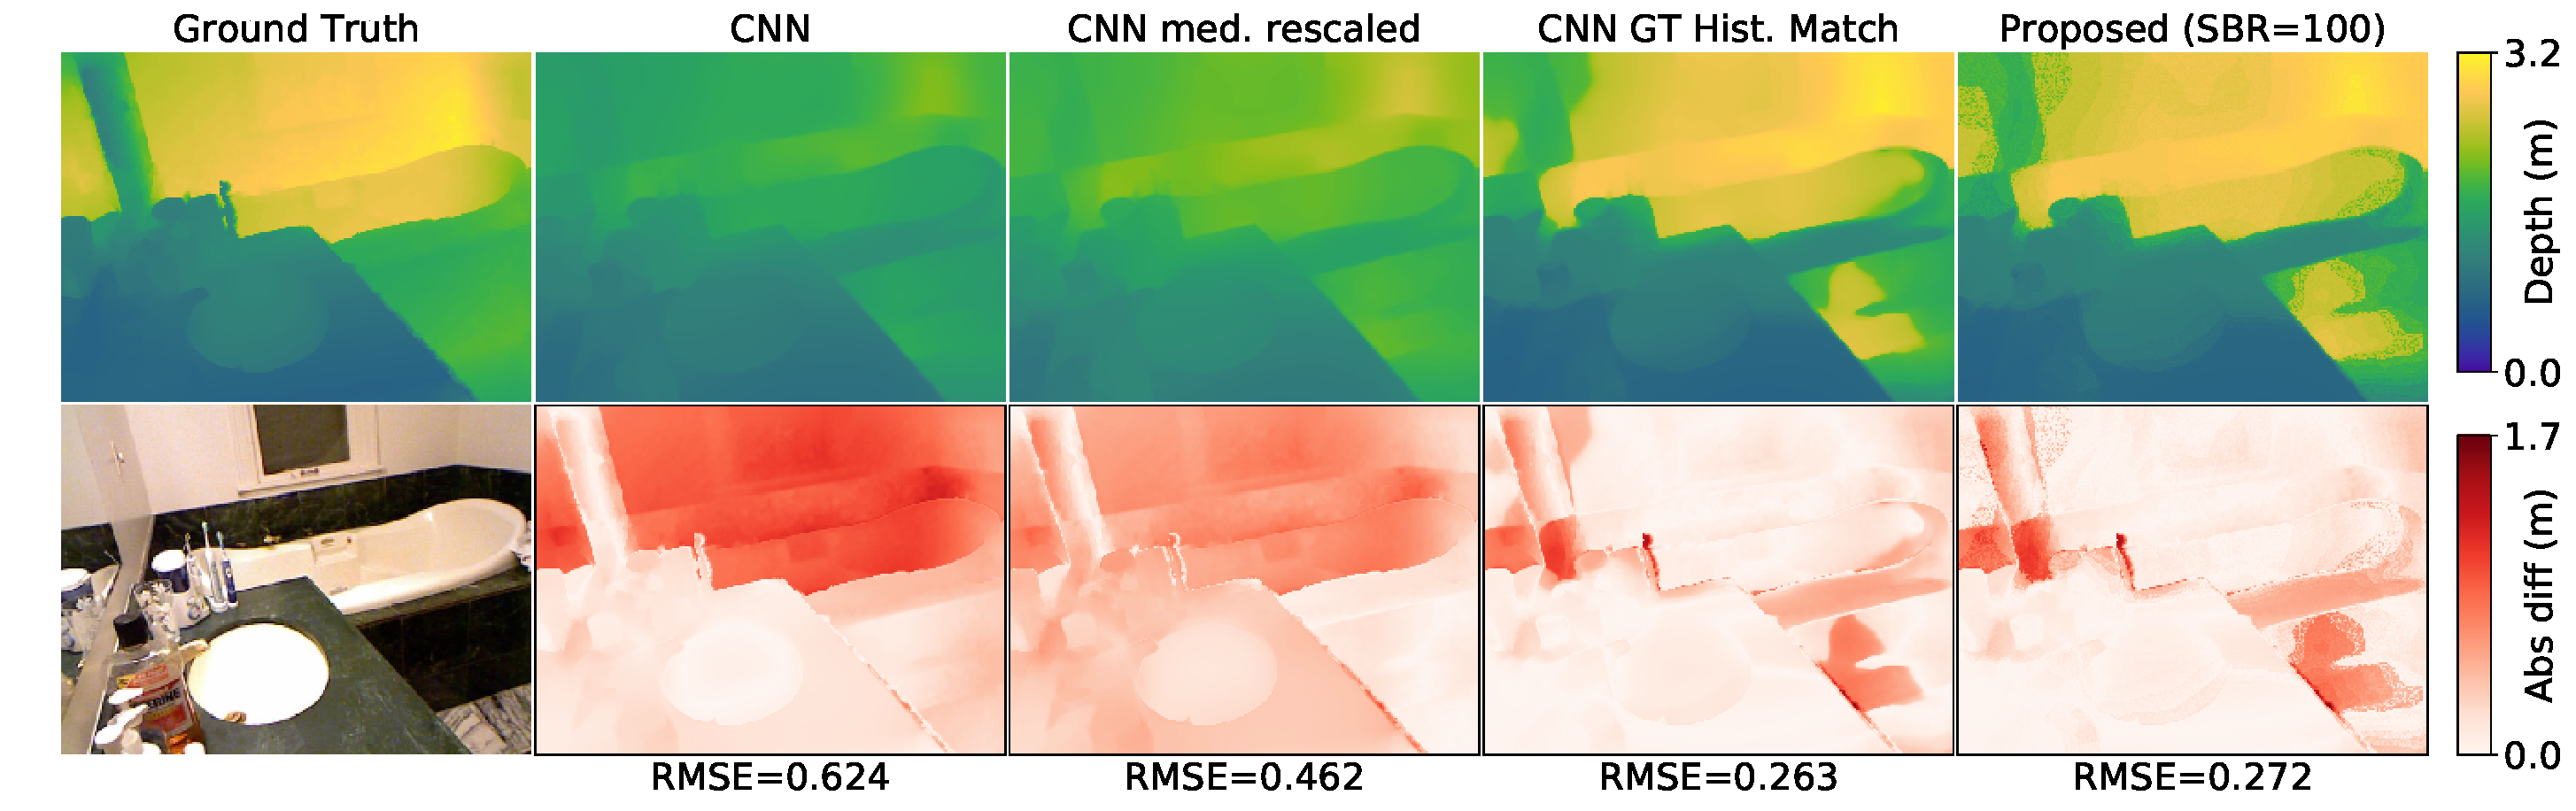
\includegraphics[width=\textwidth]{comparison/densedepth_194_comparison.pdf}
  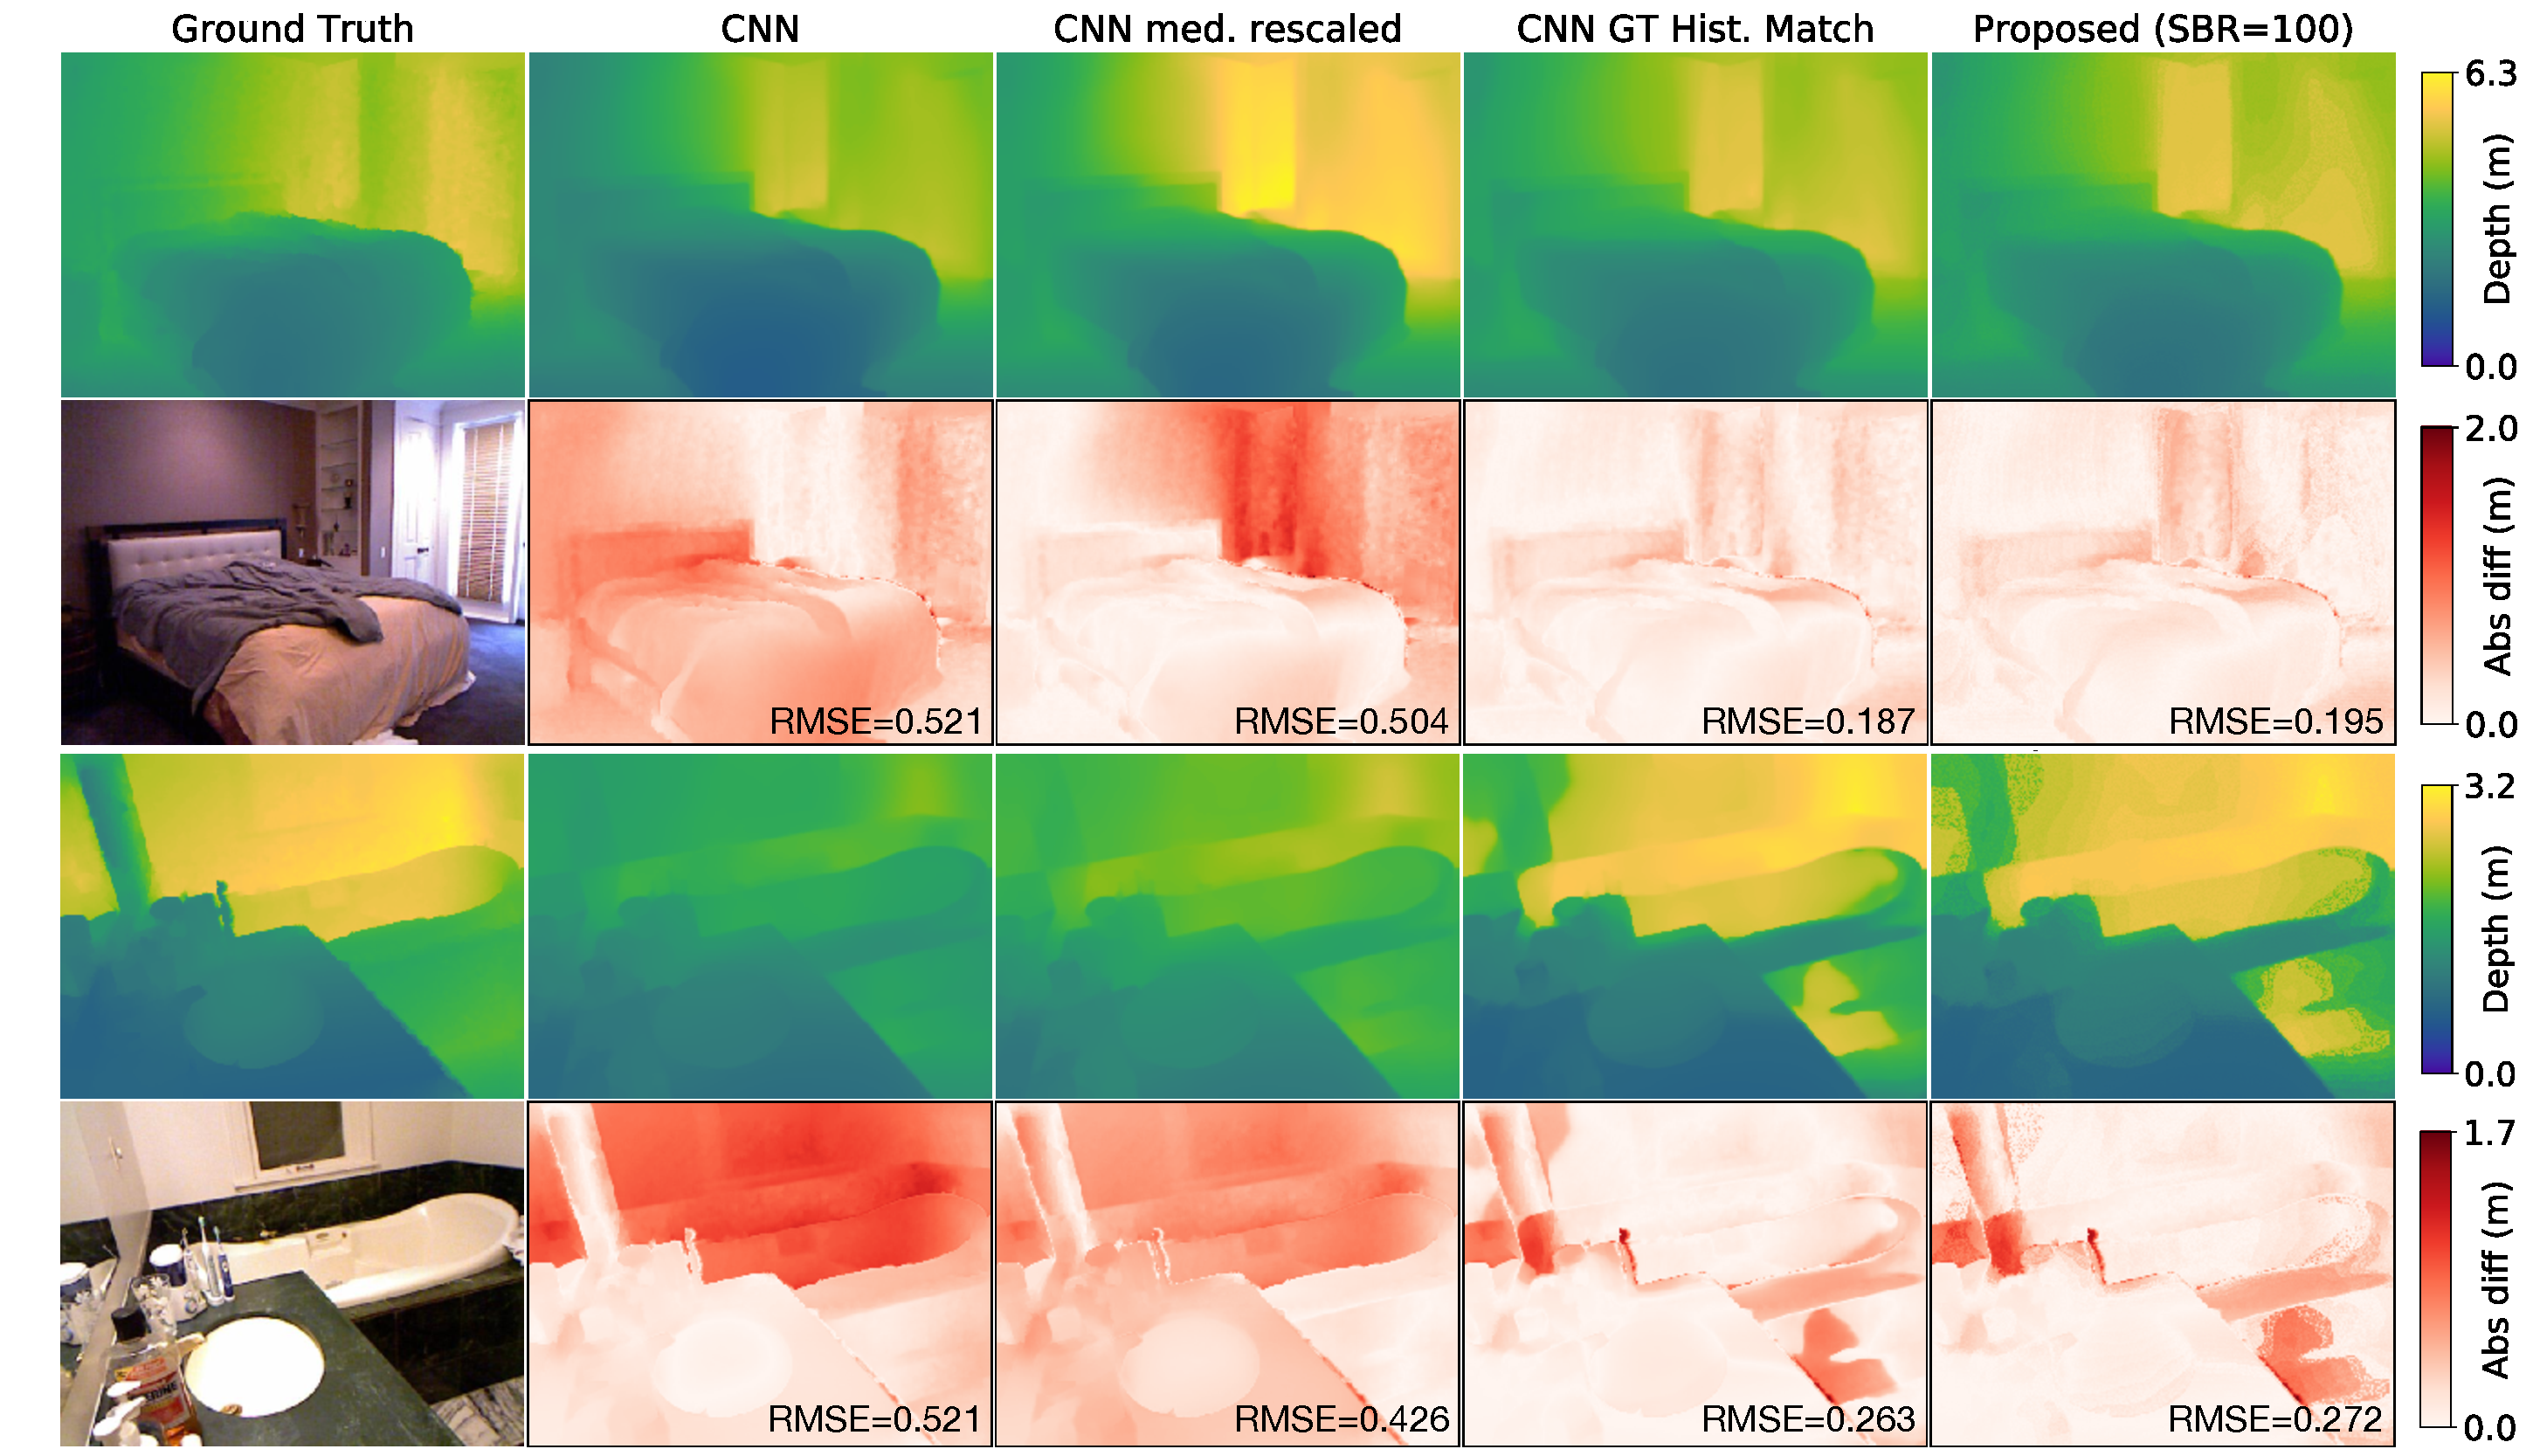
\includegraphics[width=\textwidth]{comparison.pdf}
  %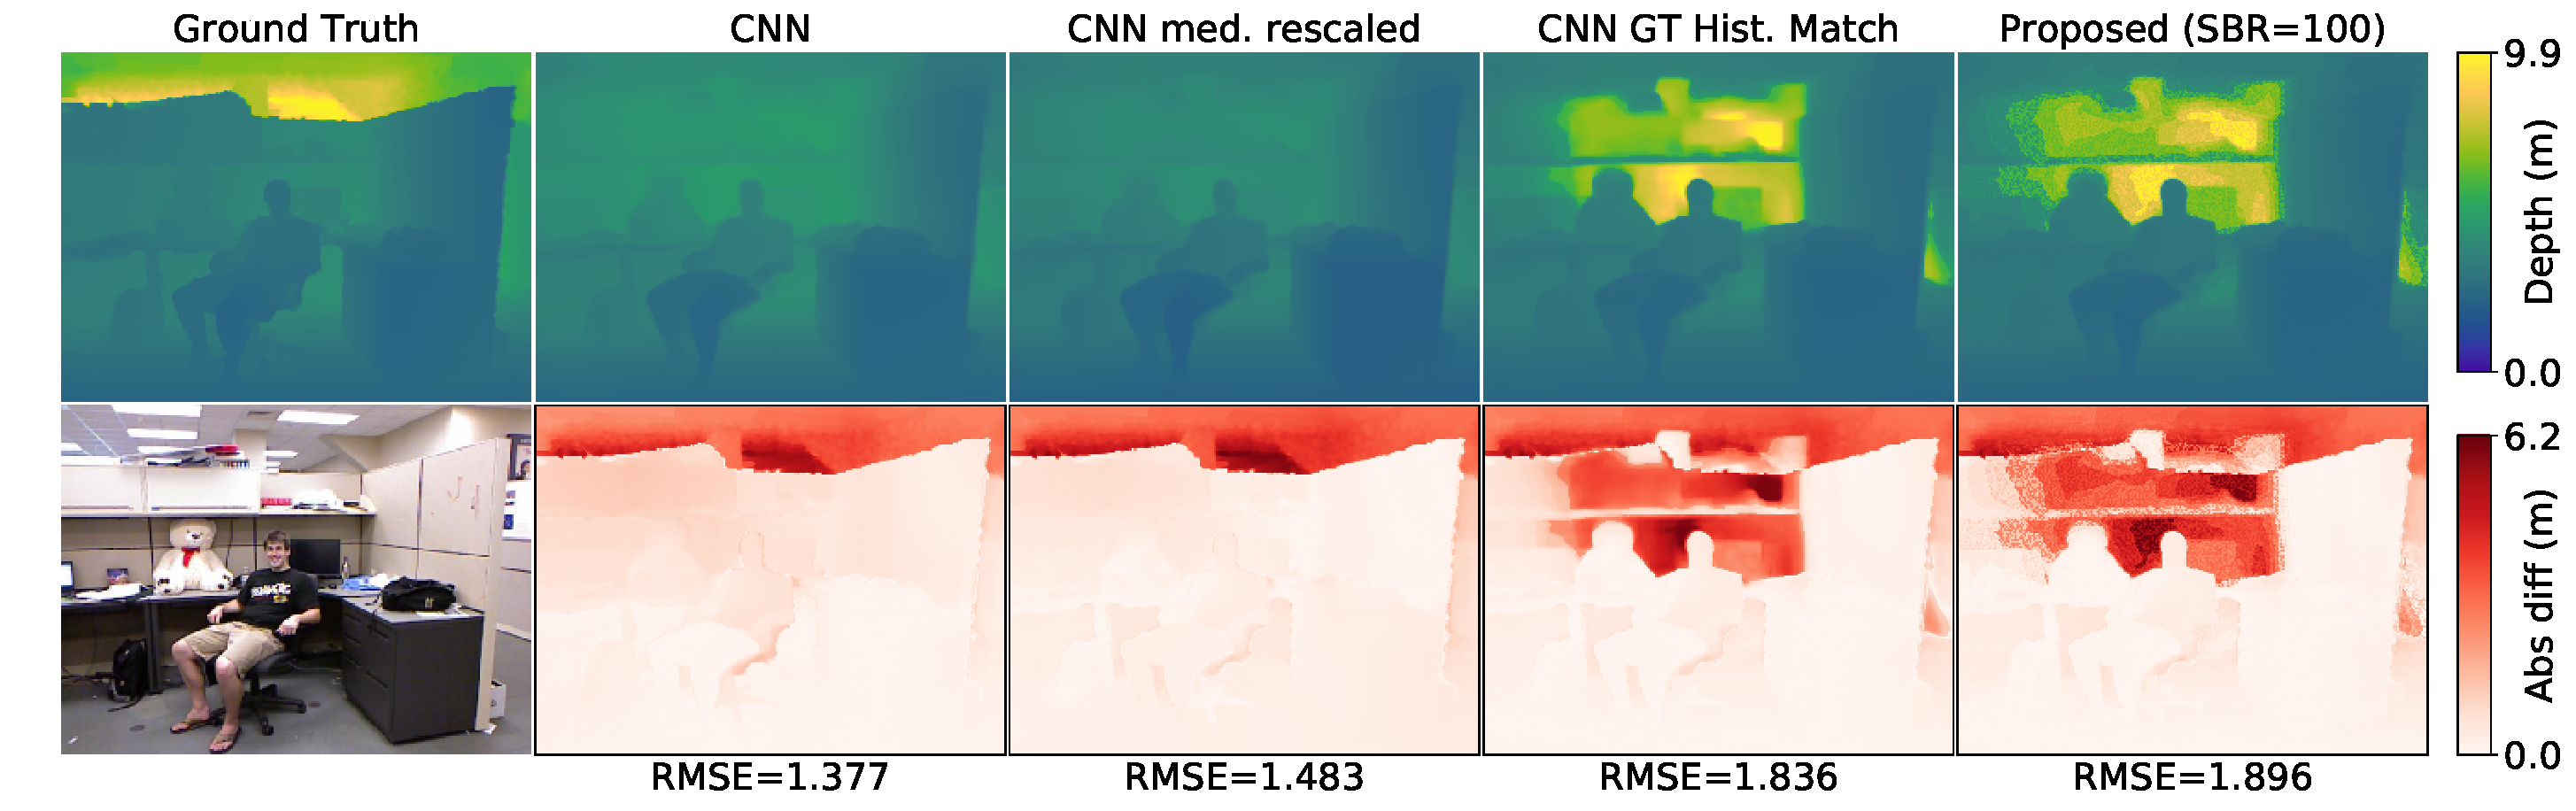
\includegraphics[width=\textwidth]{comparison/densedepth_258_comparison.png}
  \caption{Simulated results from NYU v2 computed with the DenseDepth
  CNN~\cite{Alhashim2018}. The depth maps estimated by the CNN are reasonable,
  but contain systematic error. Oracle access to the ground truth depth maps,
  either through the median depth or the depth histogram, can remove this error
  and correct the depth maps. The proposed method uses measurements from a
  single diffused SPAD and does not rely on ground truth depth, but it achieves
  a quality that closely matches the best-performing oracle.}
	\label{fig:results_simulated}
  \vspace{-1em}
\end{figure*}


%%%%%%%%%%%%%%%%%%%%%%%%%%%%%%%%%%%%%%%%%%%%%%%%%%%%%%%%%%%%%%%%%%%%%%%%%%%%%%%%%%%%%%%%%%%%%%%
\subsection{Implementation Details}

We use the NYU Depth v2 dataset to evaluate our method. This dataset consists of
249~training and 215~testing scenes with RGB-D images captured using a Microsoft
Kinect.

To simulate a SPAD histogram, we take the provided depth map and 
calculate a weighted depth histogram by weighting the pixel contributions to
each depth bin by the luminance of each pixel. To model radiometric falloff, we
multiply each bin by $1/z^2$, and convolve with a modeled system temporal
response, which we approximate as a Gaussian with a full-width at half-maximum of 70~ps. We scale
the histogram by the total number of observed signal photon counts (set to 
$10^6$) and  add a fixed number of background photons $b \in \set{10^5, 2\times
10^4, 10^4}$. The background counts are evenly distributed across all bins to simulate the ambient and dark
count detections, and the different background levels correspond to
signal-to-background ratios (SBR) of $10, 50$ and $100$ respectively. Finally,
each bin is Poisson sampled to produce the final simulated SPAD transient.

% \textcolor{red}{Need more details: how did you simulate the SPAD measurements from this: discuss albedo, square distance falloff, Poisson noise, background, number of SPAD bins, define what SBR is etc.}

%%%%%%%%%%%%%%%%%%%%%%%%%%%%%%%%%%%%%%%%%%%%%%%%%%%%%%%%%%%%%%%%%%%%%%%%%%%%%%%%%%%%%%%%%%%%%%%
\subsection{Simulated Results}

We show an extensive quantitative evaluation in Table~\ref{tab:comparison}.
Here, we evaluate three recent monocular depth estimation techniques:
DORN~\cite{Fu2018}, DenseDepth~\cite{Alhashim2018}, and
MiDaS~\cite{Lasinger:2019}. To evaluate the quality of DORN and DenseDepth, we
report various standard error metrics. Moreover, we show a simple
post-processing step that rescales their outputs by the median ground truth
depth~\cite{Alhashim2018}. We also show the results of histogram matching the
output of the CNNs with the ground truth depth map histogram. Note that we do
not report the quality of the direct output of MiDaS as this algorithm does not
output metric depth. However, we do show its output histogram matched with the
ground truth depth map histogram. In all cases, post-processing the estimated
depth maps either with the median depth or depth histogram significantly
improves the absolute depth estimation, often by a large margin compared to the
raw output of the CNNs. Unfortunately, ground truth depth is typically not
accessible so neither of these two post-processing methods are viable in
practical application scenarios.

Instead, our method uses the simulated measurements from a single diffused SPAD
to correct the depth map. In Table~\ref{tab:comparison}, results are shown for several different
signal-to-background ratios (SBRs). We see that the proposed method achieves
high-quality results for correcting the raw depth map estimated by the
respective CNNs for all cases. The quality of the resulting depth maps is almost
as good as that achieved with the oracle ground truth histogram, which can be
interpreted as an approximate upper bound on the performance, despite a
relatively high amount of noise and background signal. These results demonstrate
that the proposed method is agnostic to the specific depth estimation CNN
applied to get the initial depth map and that it generally achieves significant
improvements in the estimated depth maps, clearly surpassing the variation in
performance between depth estimation CNNs.


In Figure~\ref{fig:results_simulated}, we also show qualitative results of our
simulations. For each of these scenes, we show the RGB reference image, the
ground truth depth map, the raw output of the DenseDepth CNN, the result of
rescaling the CNN output by the median ground truth depth, the result of
histogram-matching the CNN output by the ground truth depth map histogram, and
the result achieved by the proposed method for an SBR of 100. Error maps for all
the depth estimation methods are shown. As expected, the CNN outputs depth maps
that look reasonable but that have an average root mean squared error (RMSE) of
about 50--60~cm. Re-scaling this depth map by the median ground truth depth
value slightly improves the quality and histogram-matching with the ground
truth depth histogram shows a large amount of improvement. The quality of the
proposed method is close to using the oracle histogram, despite relying on
noisy SPAD measurements. Additional simulations using DenseDepth and other depth
estimation CNNs for a variety of scenes are shown in the supplement.


